\documentclass[10pt]{article}
\usepackage[margin=1in]{geometry}
\usepackage[shortlabels]{enumitem}
%\setcounter{secnumdepth}{0}
\usepackage{amssymb,amsmath,amsthm}
\usepackage{graphicx}
\usepackage{caption}
\usepackage{fancyhdr, lastpage}
\pagestyle{fancy}
\fancyhf{}
\lhead{Daniel Standage}
\chead{GDCB 511, 9:00am MWF}
\rhead{Lecture Notes: 17-20 Feb, 2012}
%\cfoot{Page \thepage{} of \protect\pageref*{LastPage}}
\usepackage{varioref}
\labelformat{equation}{(#1)}
\usepackage[colorlinks,linkcolor=blue]{hyperref}

\newenvironment{mitemize}
{
  \begin{itemize}
  \setlength{\itemsep}{1pt}
  \setlength{\parskip}{0pt}
  \setlength{\parsep}{0pt}}{\end{itemize}
}

\newenvironment{menumerate}
{
  \begin{enumerate}
  \setlength{\itemsep}{1pt}
  \setlength{\parskip}{0pt}
  \setlength{\parsep}{0pt}}{\end{enumerate}
}

\newcommand{\textsup}[1]{\ensuremath{^{\textrm{#1}}}}
\newcommand{\textsub}[1]{\ensuremath{_{\textrm{#1}}}}


\begin{document}

\section*{Histones}
5 primary types of histones in eukaryotes
\begin{mitemize}
  \item H1
  \item H2A
  \item H2B
  \item H3 (highly conserved)
  \item H4 (highly conserved)
  \item histone tails are targets for many modifications that alter histone structure
\end{mitemize}

\subsection*{Chromatin folding}
\begin{menumerate}
  \item string of nucleosomes (nucleosome filament)
  \item filament is further folded into 30-nm fiber
  \item fiber forms loops, centered to the central matrix of chromosomes
\end{menumerate}

\subsection*{Effects of histones on transcription}
\begin{mitemize}
  \item core histones repress transcription
  \item H1 causes further repression
  \item repression counteracted by transcription factors
  \item TFs can recruit transferases to modify histones
  \item nucleosome positioning is important for gene expression
\end{mitemize}

\subsection*{Chromatin modification}
We will focus on specific modifications to the tails of H3/H4 histones
\begin{mitemize}
  \item acK (lysine acetylation)
  \item meR (arginine methylation)
  \item meK (lysine methylation)
  \item PS (serine phosphorylation)
  \item UK (lysine ubiquitination)
\end{mitemize}

\subsection*{Histone code}
\begin{mitemize}
  \item one histone modification can influence other 
  \item histone code: a combination of histone modifications that determine gene activities by helping to form euchromatin (active) or heterochromatin (inactive) states
  \item can be translated by bromodomain 
  \begin{mitemize}
    \item interacts with acetylated lysine
    \item BRG1 (SWI/SNF):H4 K8 
    \item TAF250 (TFIID): H3 K9K14
    \item bromo-HATs (GCN5, PCAF, TAF250)
  \end{mitemize}
  \item can be translated by chromodomain
  \begin{mitemize}
    \item targets methylation marks
    \item HP1 (methylated K9), repression
    \item SUV39 HMT (interacts with HP1)
    \item chromo-HATs (ESA1), activation
  \end{mitemize}
  \item Other domain
  \begin{mitemize}
    \item PHD (TAF3 or TAF110), 
    \item Recognizes H3K4me3 activation
  \end{mitemize}
\end{mitemize}

\subsection*{Chromatin remodeling}
\begin{mitemize}
  \item disrupt the core histones in nucleosomes (ATP-dependent)
  \item may also move nucleosomes
  \item create nucleosome-free enhancers with histone acetylases and other proteins
\end{mitemize}

\subsection*{Need to memorize}
\begin{center}
  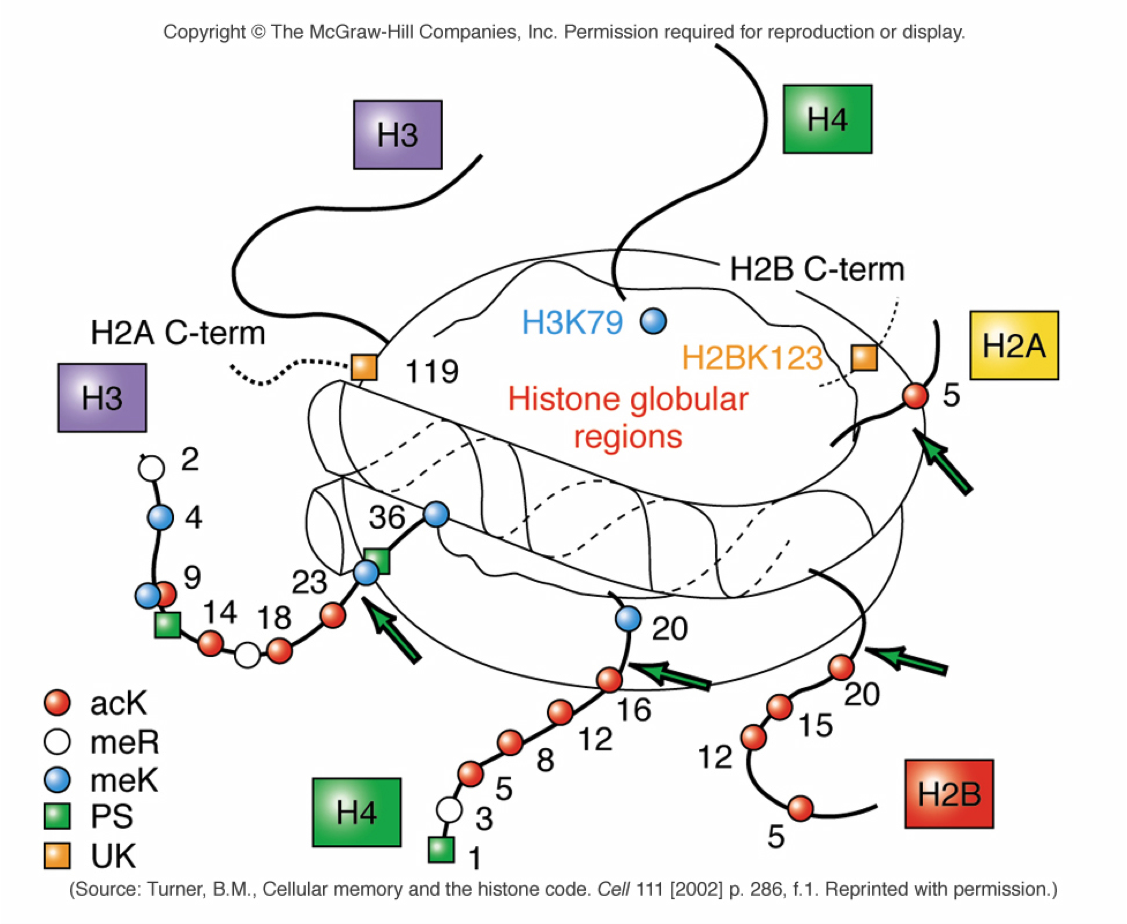
\includegraphics{histonecode.png}
\end{center}

\end{document}
